\section{Construcción del grafo bipartito}

\begin{frame}{Representación del grafo bipartito}
    \begin{itemize}
        \item<1-> Utilizamos la biblioteca Boost Graph para la representación del grafo bipartito.
        \item<2-> La BGL ofrece dos clases para representar grafos: adjacency\_list y adjacency\_matrix.
        \item<3-> La adjacency\_list resulta más conveniente que la adjacency\_matrix para nuestro caso. 
        \begin{itemize}
            \item<4-> Mejor complejidad espacial: $O(V+E)$ contra $O(V^{2})$.
            \item<5-> Recorrido de aristas salientes de un vértice más eficiente: $O(V+E)$ contra $O(V^{2})$.
            \item<6-> Más eficiente para el caso de grafos ralos.
        \end{itemize}
    \end{itemize}
\end{frame}

\begin{frame}[fragile]{Definición del grafo}
   \fontsize{9pt}{7.2}\selectfont
    \begin{lstlisting}
struct VertexProperties {
    MMO_EquationList eqs;
    AST_ExpressionList unknowns;
};

typedef boost::adjacency_list<boost::listS,
        boost::listS,
        boost::undirectedS,
        VertexProperties> CausalizationGraph;

typedef CausalizationGraph::vertex_descriptor Vertex;

typedef CausalizationGraph::edge_descriptor Edge;
    \end{lstlisting}
\end{frame}

\begin{frame}[fragile]{Construcción del grafo a partir de un modelo Modelica}
    A partir del AST y de la tabla de símbolos  del modelo identificamos las ecuaciones, las incógnitas y en qué ecuación aparece cada incógnita.
    \pause
    \begin{itemize}
        \item<2-> Expandimos las ecuaciones de tipo \verb+For-Equation+.
        \begin{lstlisting}[language=Modelica]
            for i in 1:10 loop
                a[i] = i;
            end for;
        \end{lstlisting}
        \item<3-> Idenficamos las incógnitas recorriendo la tabla de símbolos.
        \begin{itemize}
            \item Es una variable continua.
            \item No es un estado.
            \item Es la derivada temporal de una variable.
        \end{itemize}
        \item<4-> "Trazamos" las aristas del grafo determinando en qué ecuación ocurre cada variable.
    \end{itemize}
\end{frame}

\section{Aplicación del Algoritmo de Tarjan}

\begin{frame}[fragile]{Aplicación del Algoritmo de Tarjan}
    \begin{itemize}
        \item<1-> Utilizamos la función \verb+checked_edmonds_maximum_cardinality_matching+ provista por la BGL para el cálculo de matching.
        \item<2-> Construimos el grafo dirigido.
        \item<3-> Utilizamos la función \verb+strong_components+ de la BGL.
    \end{itemize}
\end{frame}

\begin{frame}[fragile]{Complejidad}
    \note{
        Matching: $O(V\times E)$ -> $E\geqslant\dfrac{V}{2}$\\
        $O(\dfrac{E}{V})$ expresa la complejidad temporal de las operaciones que recorren la lista de adyacencia de un vértice. Para grafos ralos $\dfrac{E}{V}$ es mucho más chico que $V$ y puede ser considerado constante.\\
    }
    \begin{itemize}
    \item \verb+checked_edmonds_maximum_cardinality_matching+: $O(V^{2})$.
    \item La construcción del grafo dirigido: $O(V)$.
    \item \verb+strong_components+: $O(V+E)$.
    \end{itemize}
\end{frame}

\section{Optimización del Proceso de Causalización}

\begin{frame}{Un algritmo simple para obtener la causalización de un modelo DAE sin bucles}
    \begin{itemize}
        \item Si una ecuación posee una sola incógnita, entonces debemos utilizar esa ecuación para resolver esa incógnita.
        \item Si una incógnita aparece en una sola ecuación, entonces no tenemos más alternativa que utilizar esa ecuación para resolver esa incógnita.
    \end{itemize}
\end{frame}

\begin{frame}
    \only<1>{
        \includegraphics[width=0.8\textwidth]{graphics/ej_alg_simple_op_1.png}
    }
    \only<2>{
        \includegraphics[width=0.8\textwidth]{graphics/ej_alg_simple_op_2.png}
    }
    \only<3>{
        \includegraphics[width=0.8\textwidth]{graphics/ej_alg_simple_op_3.png}
    }
    \only<4>{
        \centering
        \includegraphics[width=0.3\textwidth,height=0.7\textheight]{graphics/ej_alg_simple_op_4.png}
    }
\end{frame}

\section{Ejemplo}

\begin{frame}[fragile]{Circuito RLC}
   \fontsize{8pt}{7.2}\selectfont
    \begin{columns}
        \begin{column}{0.5\textwidth}
        \begin{lstlisting}[language=Modelica]
model RLC
    Real u1; Real u2;
    Real uL; Real iC;
    Real i1; Real i2;
    Real u0; Real i0;
    Real iL; Real uC;
    parameter Real R1;
    parameter Real R2;
    parameter Real L;
    parameter Real C;
    equation
        u0 = sin(time);
        u1 = R1 * i1;
        u2 = R2 * i2;
        uL = L * der(iL);
        iC = C *der(uC);
        u0 = u1 + uC;
        uL = u1 + u2;
        uC = u2;
        i0 = i1 + iL;
        i1 = i2 + iC;
end RLC;
        \end{lstlisting}
        \end{column}
        \begin{column}{0.5\textwidth}
        \begin{lstlisting}[language=Modelica]
model RLC
    Real u1; Real u2;
    Real uL; Real iC;
    Real i1; Real i2;
    Real u0; Real i0;
    Real iL; Real uC;
    parameter Real R1;
    parameter Real R2;
    parameter Real L;
    parameter Real C;
    equation
        u0 = sin(time);
        u2 = uC;
        u1 = (-uC)+u0;
        i2 = u2*(1/(R2));
        i1 = (1/(R1))*u1;
        iC = (-i2)+i1;
        uL = u1+u2;
        der(uC) = iC*(1/(C));
        der(iL) = (1/(L))*uL;
        i0 = i1+iL;
end RLC;
        \end{lstlisting}
        \end{column}
    \end{columns}
\end{frame}

\section{Prueba de Eficiencia}

\begin{frame}{Transmisión de energía en una dimensión}
    \begin{center}
        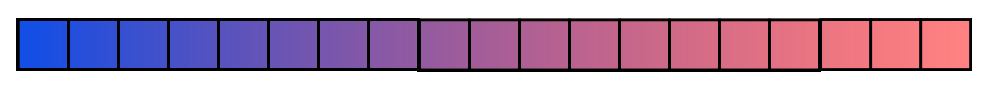
\includegraphics[width=0.8\textwidth]{graphics/heat_transfer.eps}
    \end{center}
    \pause
    \begin{eqnarray*}
        \dot{u}_{n}(t) & = & 0\\
        \dot{u}_{1}(t) & = & \frac{u_{1}(t)-u_{2}(t)}{\frac{1}{N}}\\
        \dot{u}_{i}(t) & = & \frac{u_{i+1}(t)-u_{i}(t)}{\frac{1}{N}}+\frac{u_{i-1}(t)-u_{i}(t)}{\frac{\gamma}{N}}\;
    \end{eqnarray*}
\end{frame}

\begin{frame}[fragile]{Modelo Modelica}
\fontsize{8pt}{7.2}\selectfont
\begin{lstlisting}[language=Modelica]
  model OneDHeatTransferTI_FD
    parameter Real L = 0.2;
    constant Integer N = 100;
    parameter Real T0 = 273.15;
    parameter Real TN = 330;
    parameter Real cp = 910;
    parameter Real lambda = 237;
    parameter Real rho = 2712;
    final parameter
    Real dx = L / (N - 1);
    Real T[N];
    equation
      der(T[N]) = 0;
      for i in 2:N - 1 loop
        der(T[i]) = lambda * ((T[i + 1] - T[i]) / dx + ((-T[i]) + T[i - 1]) / dx) / cp / rho / dx;
      end for;
      der(T[1]) = lambda * ((T[2] - T[1]) / dx) / cp / rho / dx;
  end OneDHeatTransferTI_FD; 
\end{lstlisting}
\end{frame}

\begin{frame}{Resultados Caso 1}
\begin{center}
\includegraphics[width=0.8\textwidth]{graphics/OneDHeatTransfer.png}
\end{center}
\end{frame}

\begin{frame}[fragile]{Modelo Modelica con Bucle Algebraico}
\fontsize{8pt}{7.2}\selectfont
\begin{lstlisting}[language=Modelica]
  model OneDHeatTransferTI_FD
    ...
    Real T[N];
    Real U[N]; 
    equation
      der(T[N]) = 0;
      U[1]*U[2]=0;
      for i in 2:N - 1 loop
        der(T[i]) = der(T[i-1]) + lambda * ((T[i + 1] - T[i]) / dx + ((-T[i]) + T[i - 1]) / dx) / cp / rho / dx;
        U[i] = U[i+1]+U[i-1]; 
      end for;
      der(T[1]) = lambda * ((T[2] - T[1]) / dx) / cp / rho / dx;
      U[N] = U[N-1]*2+sin(U[N]); 
  end OneDHeatTransferTI_FD; 
\end{lstlisting}
\end{frame}

\begin{frame}{Resultados Caso 2}
\begin{center}
\includegraphics[width=0.8\textwidth]{graphics/OneDHeatTransfer_loop.png}
\end{center}
\end{frame}

\section{Conclusiones}

\begin{frame}{Conclusiones}
    \begin{itemize}
        \item<1-> Presentamos la implementación en C++ de la etapa de causalización de eucaciones de un compilador modelica.
        \item<2-> Estudiamos e implementamos tres estrategias distintas para resolver el problema de causalización analizando la complejidad computacional de cada una de ellas.
        \item<3-> Utilizamos bibliotecas abiertas como la BGL o GiNaC.
        \item<4-> Utilizando ejemplos del dominio de la ingenería electrica probamos que algoritmo de causalización produce resultados correctos para casos con y sin bucles algebraicos.
        \item<5-> Analizamos el desempeño de las diferentes estrategías utilizando un modelo de grande.
    \end{itemize}
\end{frame}

\begin{frame}[fragile]{Trabajo a futuro}
    \note{
        Singularidad estructural: Un modelo presenta singularidades estructurales si el orden del sistema
    }
    \begin{itemize}
        \item Implementación del algoritmo de Pantelides para eliminar las singularidades estructurales.
        \item Tratamiento de los lazos algebraicos mediante la técnica de Tearing.
        \item Causalización de ecuaciones de tipo \verb+For-Equation+ sin realizar la expansión del For.
    \end{itemize}
\end{frame}

